\chapter{Experiments and Methods}\label{chapter:experiments}
In the beginning of the chapter, the synthetically generated dummy and real-world BSD datasets are presented. In the course of that, the experimental setup, data recording, domain shift and classification problem is described. In the end the proposed model architecture as well as the corresponding training are described. 
\section{Dummy Dataset}
As a first evaluation, different MMD-based domain adaptation approaches for PHM applications were evaluated on a synthetically generated dummy dataset. Such datasets are structured equally and show similar patterns as the corresponding real-world datasets. The complexity in such datasets and therefore the difficulty of the corresponding tasks can be tuned arbitrarily. When applying new and unknown methods, dummy datasets can help to understand their underlying mechanisms and effects on the data-level. Besides that, they serve as a prior evaluation of the approach's applicability for the corresponding real-world task. A simple dummy dataset, containing a domain shift, was established to evaluate, how MMD-losses can optimize neural networks to extract more domain invariant features. Since one has to deal with irregularities, outliers and noise in real-world data, it is helpful to evaluate the MMD-loss on a dataset, which is not disturbed by these effects. Similarly to PHM applications, the dummy dataset contained one-dimensional time sequences, each containing 1000 data points. In order to simulate a classification problem with two classes and two domains, the data points of each sequence were sampled from four cosine curves with characteristic amplitudes and frequencies. By adjusting the amplitude and frequency, the domain adaptation problem can be configured more or less difficult. The sampling process included a certain randomness to allow variations between sequences of the same class and domain. For every sampling step, the characteristic amplitude and frequency of the cosine curve was perturbed. This changed the underlying characteristic of each sequence. Besides that, noise was added to each of the 1000 data points. This is necessary to generate a periodic signal which is close to a noisy real-world vibration signal. Exemplary samples for both classes and domains are shown in fig. \ref{fig:samples_domain_class_dummy}.

\begin{figure}[H]
  \centering
  \includegraphics[width=.45\textwidth]{samples_domain_class_dummy/Source_Domain_Class_0_obs_0.pdf}
  \hspace{.3cm}
  \includegraphics[width=.45\textwidth]{samples_domain_class_dummy/Source_Domain_Class_1_obs_0.pdf}

  \vspace{.3cm}

  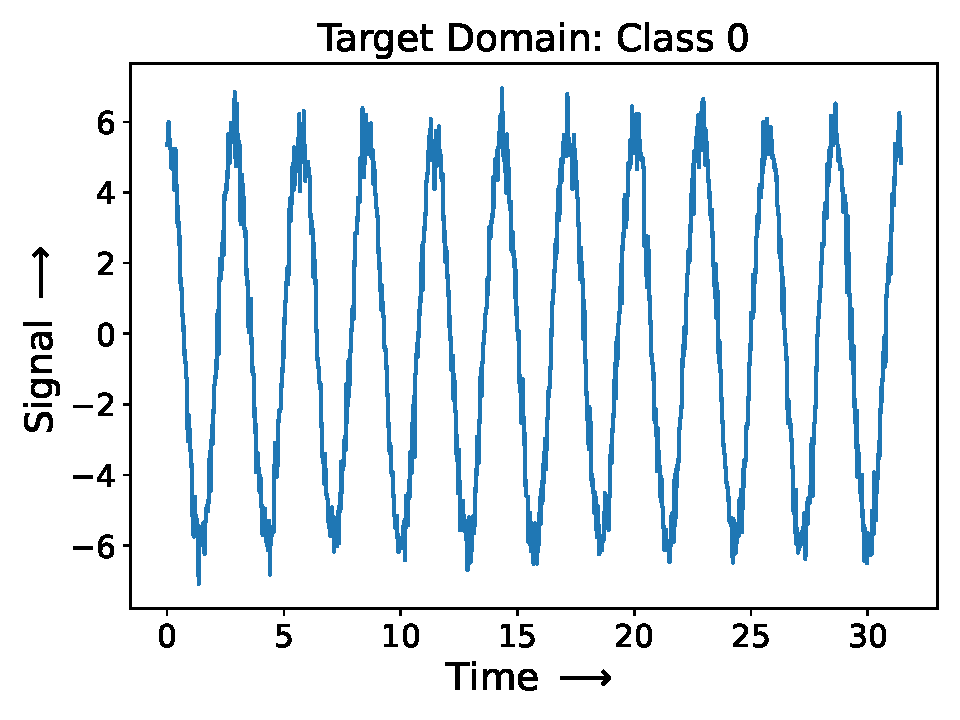
\includegraphics[width=.45\textwidth]{samples_domain_class_dummy/Target_Domain_Class_0_obs_0.pdf}
  \hspace{.3cm}
  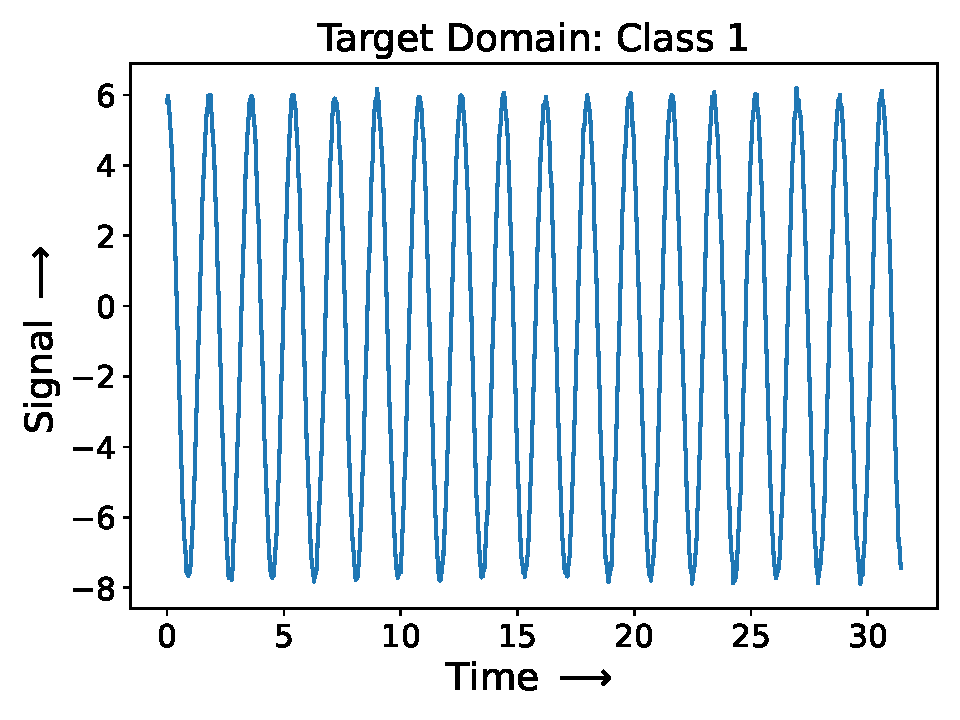
\includegraphics[width=.45\textwidth]{samples_domain_class_dummy/Target_Domain_Class_1_obs_0.pdf}

  \caption{Data window samples for each domain and class}
  \label{fig:samples_domain_class_dummy}
\end{figure}

In fig. \ref{fig:samples_domain_class_dummy_influence_noise} one can see how the perturbation and noise, applied during the sampling process, influence the data sequences. The noise, frequency and amplitude changed quite a bit between the samples belonging to the same class and domain.

\begin{figure}[H]
  \centering
  \includegraphics[width=.45\textwidth]{samples_domain_class_dummy_influence_noise/Source_Domain_Class_0_obs_0.pdf}
  \hspace{.3cm}
  \includegraphics[width=.45\textwidth]{samples_domain_class_dummy_influence_noise/Source_Domain_Class_1_obs_0.pdf}

  \vspace{.3cm}

  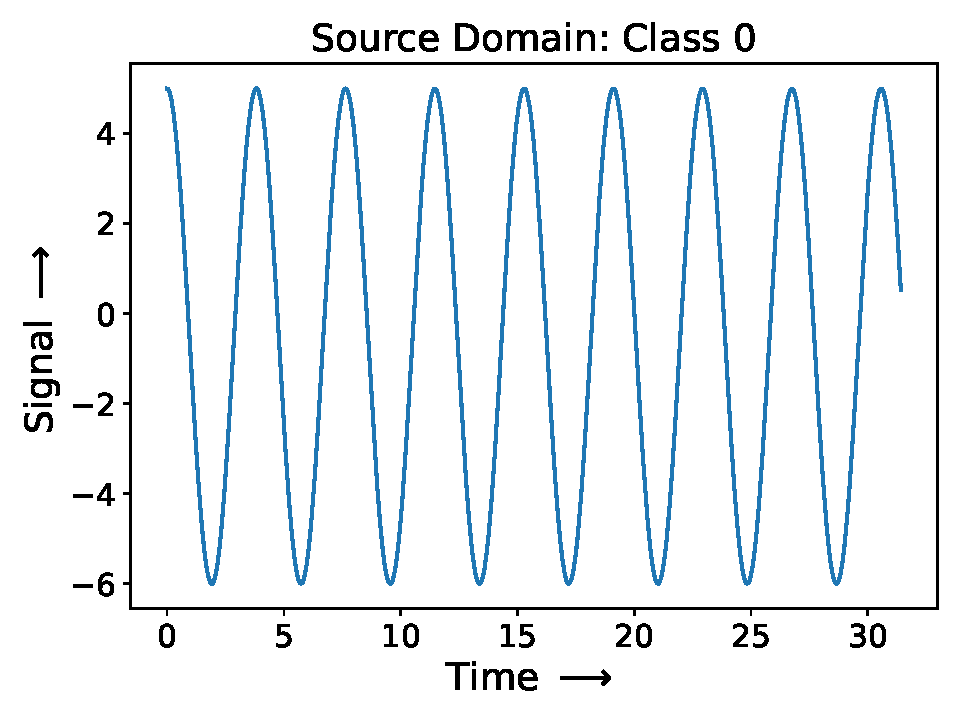
\includegraphics[width=.45\textwidth]{samples_domain_class_dummy_influence_noise/Source_Domain_Class_0_obs_1.pdf}
  \hspace{.3cm}
  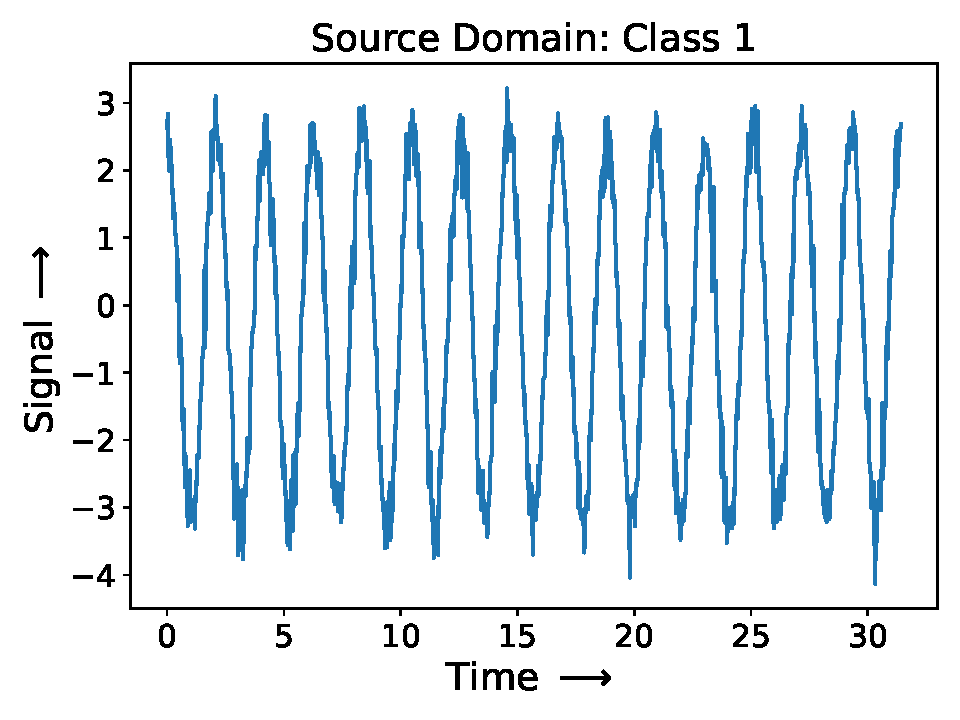
\includegraphics[width=.45\textwidth]{samples_domain_class_dummy_influence_noise/Source_Domain_Class_1_obs_1.pdf}

  \caption{Perturbation and noise during sampling process}
  \label{fig:samples_domain_class_dummy_influence_noise}
\end{figure}

\section{Dataset: Ball Screw Drive}
Testing the developed PHM methods on a real-world dataset is essential to make statements about the method's utility and applicability in the PHM of industrial machines. In the following, the data collection from a milling machine is described in detail. Milling machines are common in the industry and contain several BSDs and LGSs, which suffer from continuous degradation. A continuous evaluation of the degradation state and replacement of these components is necessary. Due the industrial relevance of BSD health monitoring, a dataset was recorded on a milling machine to evaluate the developed PHM system on a real-world scenario.

\subsection{Experimental Setup}
Data from a DMG DMC 55H duoblock milling machine of the manufacturer DMG Mori was recorded. The machine tool’s spindle and housing, as well as the machine tool table, rotatory axes, peripherals, the cladding and the machine tool's housing were removed. The TNC control iTNC530 HSCI from Heidenhain GmbH was used. Fig. \ref{fig:experimental_setup} shows the experimental setup. The investigation focused on the moving hanger assembly of the machine tool. The machine tool is generally able to move in the three spatial directions. The dataset just included data from machine tool movements along the x-axis. For this reason, just the single threaded shaft of the BSD and the two LGSs, which are responsible for movements along the x-axis, were supervised.

\begin{figure}[H]
  \centering
  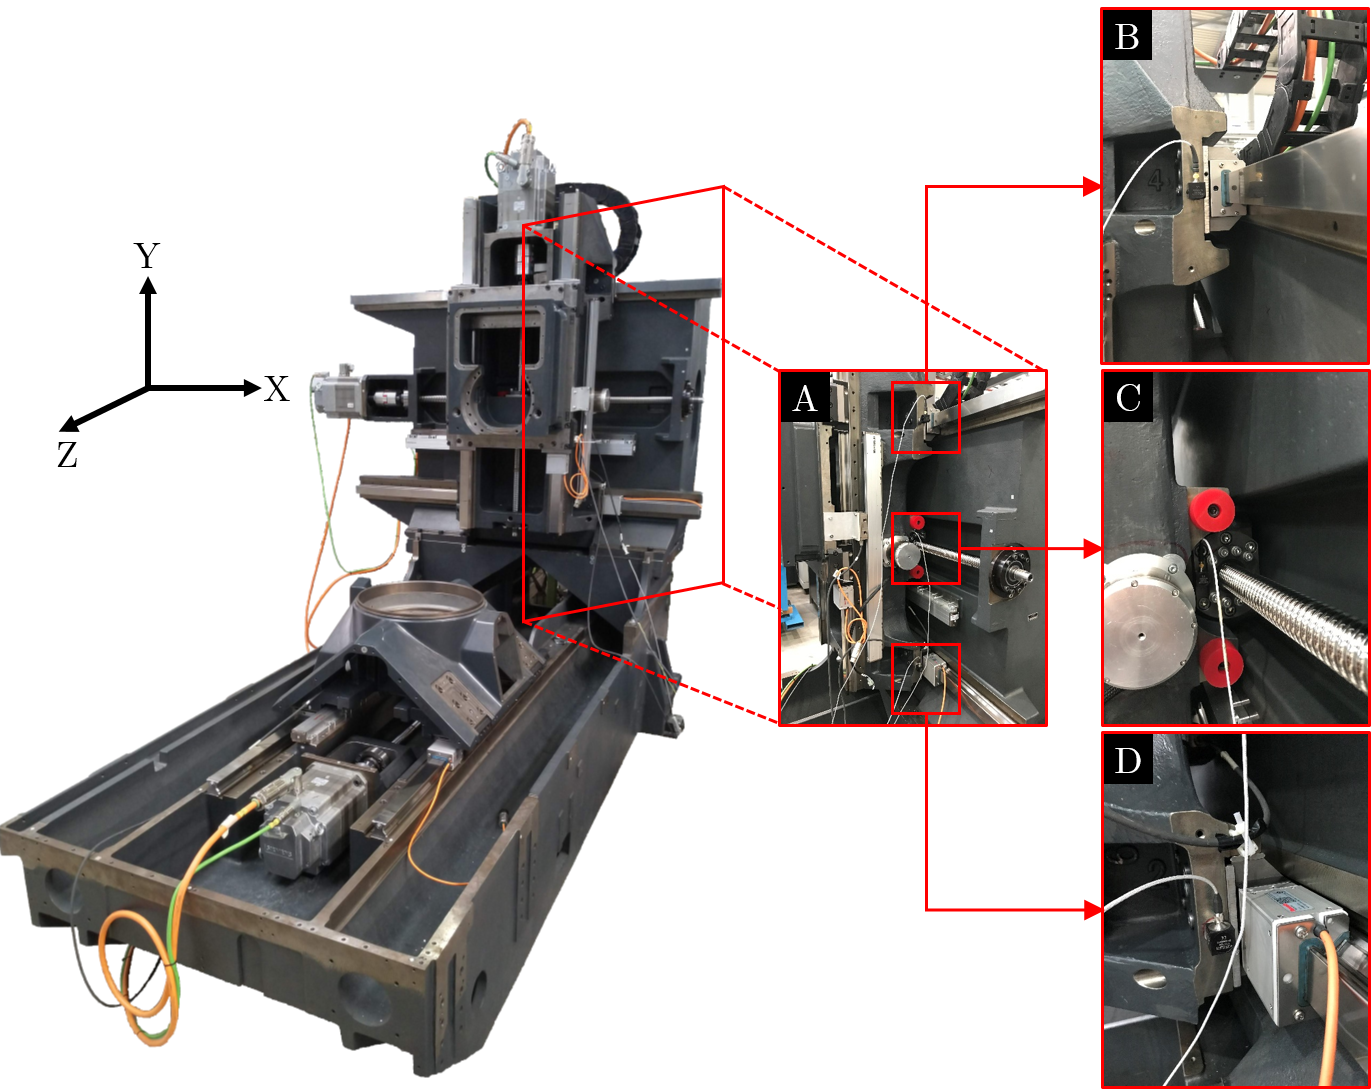
\includegraphics[width=0.9\textwidth]{experimental_setup}
  \caption {Experimental setup: s side-view of the machine, B: upper LGS, C: threaded shaft of BSD, C: lower LGS}
  \label{fig:experimental_setup}
\end{figure}

\subsection{Sensors}
The signals included in the dataset came from three different sources of measurement, the acceleration sensors and the internal control data accessed via TNC Scope and TNC Opt. The recordings of the three different sources were triggered by different software programs which were synchronized by a python script. Minor time delays between the signals could not be eliminated completely. Three triaxial Kistler 8762A10 piezo-eletric accelerometers were placed on different locations of the machine, recording accelerations in x,y,z-directions. The positions are specified in fig. \ref{fig:experimental_setup}. Accelerometers are placed at the upper LGS (sub-figure B), the BSD nut (sub-figure C) and the lower LGS (sub-figure D). The software tool TNC Scope was used to access the internal contol data of the machine. TNC Opt is a software tool, which is intended for controller optimization. During the experiments it was used to access those control data channels, which differ from those of TNC Scope.

\subsection{Definition of Degradation States}
Preload classes (C1, C2, C3) were defined, specifying the preload level in BSDs and LGSs. For the BSDs also pitting damages were observed, which is why a separate pitting class (P) was defined. The degradation of BSDs was specified by an ID containing one letter and either two digits for the preload classes or one digit for the pitting class. The degradation of LGSs was specified by an ID containing one letter and one digit. The letter indicates the damage types: no pitting (C) or pitting (P). The first digit in the BSD preload classes and the single digit in the LGS preload classes specifies the preload. The second digit in the BSD preload classes and the single digit in the BSD pitting class specifies the observation. The preload level was separated in three distinct classes. Based on the preload force (N), which was measured in the components, the recorded samples were assigned to the classes. Low preload forces are the result of high preload losses, which indicate strong component degradation. This leads to a lower machine precision and a higher risk of machine failure. Preload class C3 was labelled as “healthy”, C2 as "slightly degraded" and C1 as "strongly degraded". Two sets of BSDs and one set of LGSs, each of them containing components of all predefined health condition class, were used during the data recording. To separate equally degraded BSDs from different sets, the observation digit was included in the BSD IDs. In total, ten recordings were made for each BSD and LGS combination. Table \ref{tab:recorded_combinations_of_LGS_and_BSD_health_conditions} shows all 24 combinations of differently degraded and observed BSDs and LGSs. The forces specifying the different preload classes were defined differently for the observations. Table \ref {tab:BSDs_states} and table \ref {tab:LGSs_states} show all used BSDs and LGSs and their corresponding preload forces. Each experimental setup included two LGSs, each consisting of two counterparts, and one BSD. This is the reason, why in table \ref {tab:BSDs_states} each ID maps to one and in table \ref {tab:LGSs_states} to four preload forces.



\begin{center}
\begin{longtable}{c c c} 
\toprule
 ID & Preload in N \\ [0.5ex] 
\midrule
 P1 & 2 070 \\ 
 P2 & 2 160 \\ 
 C11 & 950 \\ 
 C12 & 845 \\ 
 C21 & 1 450 \\ [1ex] 
 C22 & 1 293 \\ [1ex] 
 C31 & 2 390 \\ [1ex] 
 C32 & 2 328 \\ [1ex] 
\bottomrule
\caption {BSDs health condition states}
\label {tab:BSDs_states}
\end{longtable}
\end{center}

\begin{center}
\begin{longtable}{c c c} 
\toprule
 ID & Component & Preload in N \\ [0.5ex] 
\midrule
 C1 & C1 & 4 060 \\ 
    & C2 & 4 430 \\ 
    & C3 & 4 430 \\
    & F1 & 3 880 \\ 
\midrule
 C2 & B1 & 8 860 \\ 
    & B2 & 9 700 \\ [1ex] 
    & B3 & 9 070 \\ [1ex]
    & E1 & 8 230 \\ [1ex]
\midrule
 C3 & A9 & 13 470 \\ 
    & A10 & 14 530 \\ [1ex] 
    & A11 & 12 840 \\ [1ex]
    & D3 & 12 840 \\ [1ex]
\bottomrule
\caption {LGSs health condition states}
\label {tab:LGSs_states}
\end{longtable}
\end{center}

\begin{comment}
\begin{center}
\begin{longtable}{c c c c c c c c c c} 
\toprule
%\multicolumn{10}{c}{BSD}
&&&&BSD&&&&
\cmidrule(lr){3-11}
  & & C31 & C21 & C11 & P1 & C22 & C12 & C32 & P2  \\ [0.5ex] 
\cmidrule(lr){3-11}
                          & C1 & 1 & 2 & 3 & 4 & 5 & 6 & 7 & 9 \\ 
LGS                       & C2 & 10 & 11 & 12 & 13 & 14 & 15 & 16 & 18  \\ 
                          & C3 & 19 & 20 & 21 & 22 & 23 & 24 & 25 & 27  \\
\bottomrule
\caption {Combinations of LGS and BSD health condition states}
\label {tab:recorded_combinations_of_LGS_and_BSD_health_conditions}
\end{longtable}
\end{center}
\end{comment}






\begin{center}
\begin{longtable}{c c c c c c c c c c} 
\toprule
  &  &    &     &     &     \multicolumn{2}{c}{BSD}     &     &     &    \\ 
  &  & C31 & C21 & C11 & P1  & C22 & C12 & C32 & P2 \\ 
\midrule
     & \multicolumn{1}{c|}{C1} & 1 & 2 & 3 & 4 & 5 & 6 & 7 & 9 \\ 
 LGS & \multicolumn{1}{c|}{C2}& 10 & 11 & 12 & 13 & 14 & 15 & 16 & 18 \\  
     & \multicolumn{1}{c|}{C3} & 19 & 20 & 21 & 22 & 23 & 24 & 25 & 27 \\ 
\bottomrule
\caption {Combinations of LGS and BSD health condition states}
\label {tab:recorded_combinations_of_LGS_and_BSD_health_conditions}
\end{longtable}
\end{center}


\subsection{Recording of Dataset}
For the sake of reproducibility, the experiments were executed with a defined test cycle, which is defined in fig. \ref{fig:test_cycle}. Machine data was collected during constant speed, direction change and sweep excitement along the machine tools X-axis. During the constant speed excitement, the machine tools were moved back and forth along the whole axis ($\Delta x$ = 600mm). During the direction change excitation, the movement of the machine tools was restricted to a small part of the axis ($\Delta x$ = 1mm) and the directions were changed with a high frequency. In the sweep excitement, the motor received a target speed in the form of a sine sweep. Before recording data, the machine was warmed up for 60min with a constant speed excitement to create equivalent circumstances for all runs.

\begin{figure}[H]
  \centering
  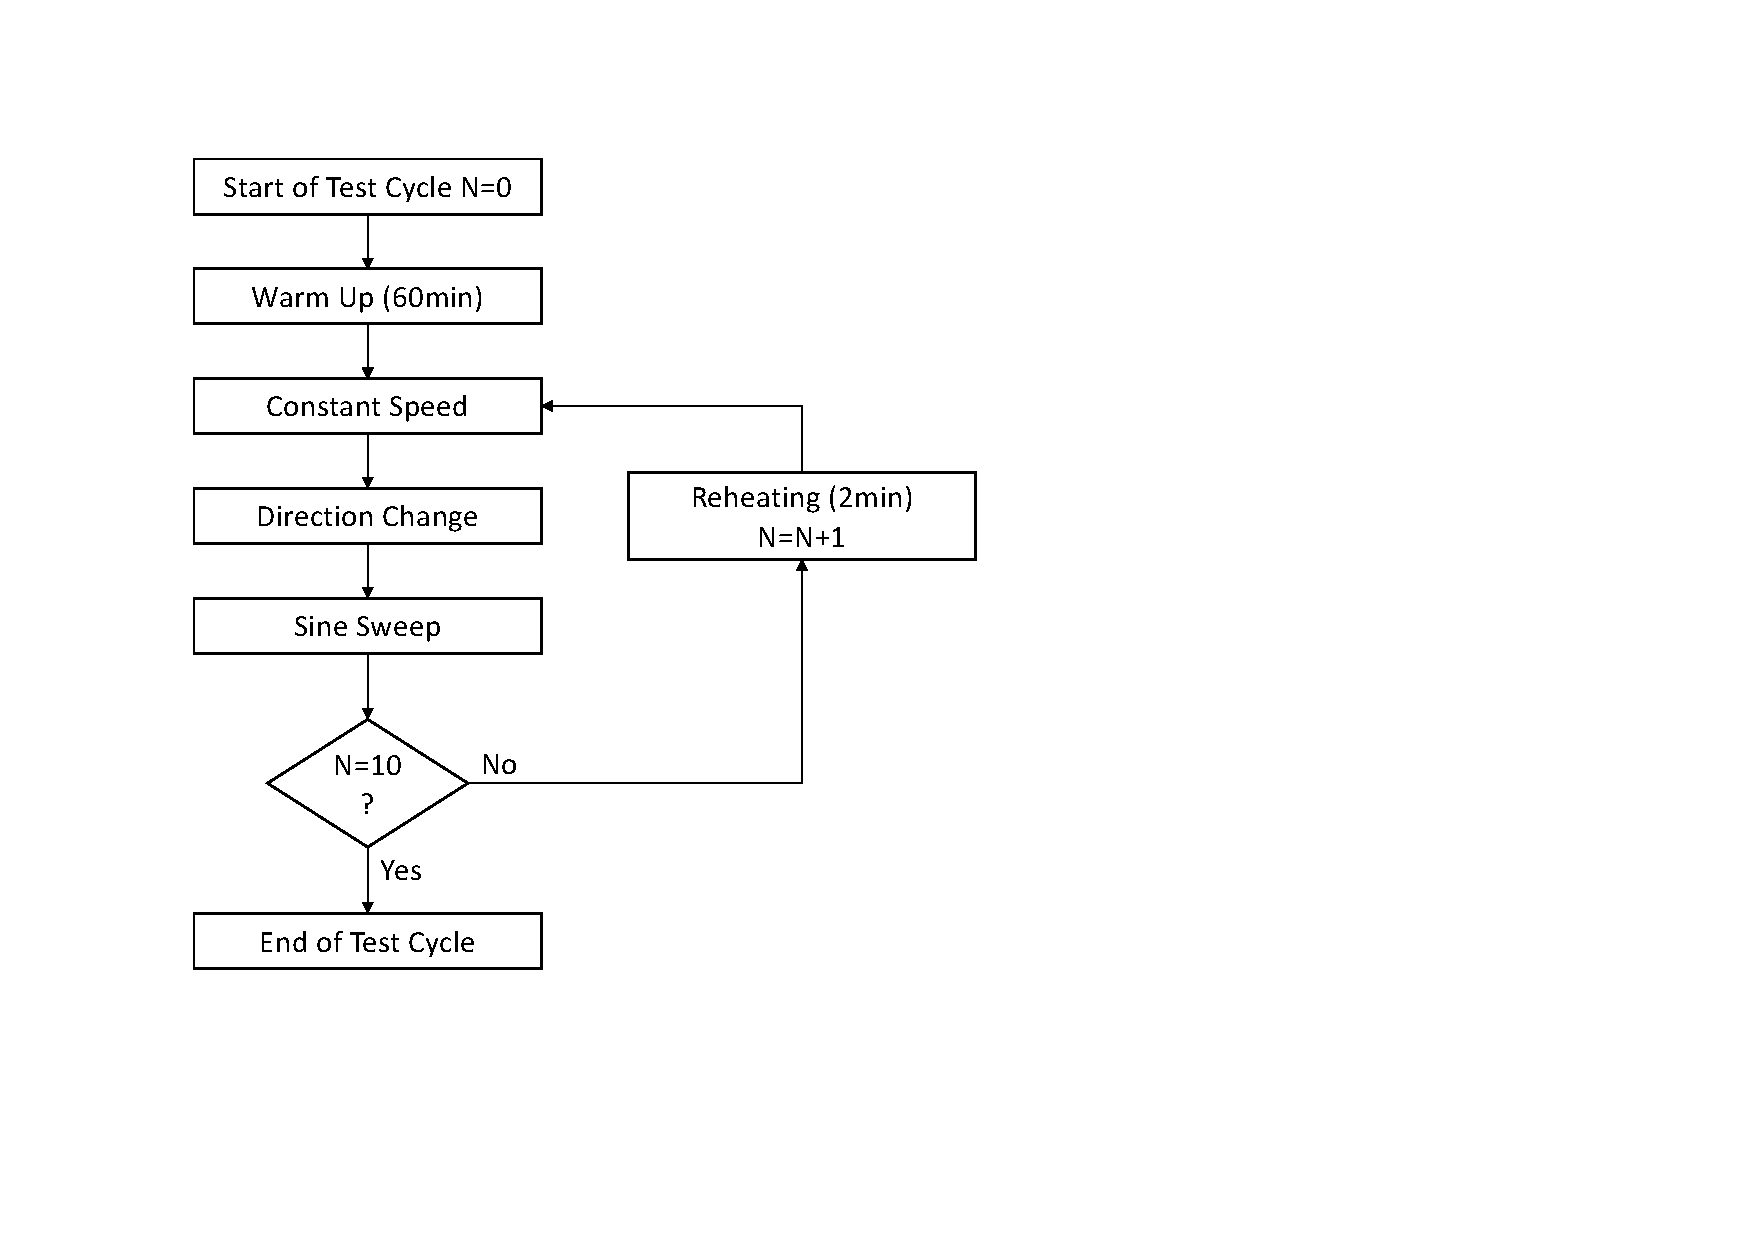
\includegraphics[width=0.7\textwidth]{test_cycle.pdf}
  \caption {Test cycle for data recording}
  \label{fig:test_cycle}
\end{figure}

In total 49 different signals were recorded. The signals are specified in more detail in table. \ref{tab:description_of_the_49_recorded_features}. All feature names starting with "C" correspond to the constant speed , "D" to the direction change and "S" to the sweep excitement.

\begin{center}
\begin{longtable}{c c c c} 
 \toprule
 Signal & Sensor & Frequency & Samples \\ [0.5ex] 
 \midrule
 C:s ist/X & TNC Scope & 10 kHz & 75000 \\ 

 C:s soll/X & TNC Scope & 10 kHz & 75000 \\ 

 C:s diff/X & TNC Scope & 10 kHz & 75000 \\ 

 C:v (n ist)/X & TNC Scope & 10 kHz & 75000 \\ 

 C:v (n soll)/X& TNC Scope & 10 kHz & 75000 \\ 

 C:P mech./X & TNC Scope & 10 kHz & 75000 \\ 

 C:Pos. Diff./X & TNC Scope & 10 kHz & 75000 \\ 

 C:I ist/X & TNC Scope & 10 kHz & 75000 \\ 

 C:I soll/X & TNC Scope & 10 kHz & 75000 \\ 

 C:x bottom & Acc & 10 kHz & 75000 \\ 

 C:y bottom & Acc & 10 kHz & 75000 \\ 

 C:z bottom & Acc & 10 kHz & 75000 \\ 

 C:x nut & Acc & 10 kHz & 75000 \\ 

 C:y nut & Acc & 10 kHz & 75000 \\ 

 C:z nut & Acc & 10 kHz & 75000 \\ 

 C:x top & Acc & 10 kHz & 75000 \\ 

 C:y top & Acc & 10 kHz & 75000 \\ 

 C:z top & Acc & 10 kHz & 75000 \\ 

 D:s ist/X & TNC Scope & 10 kHz & 75000 \\

 D:s soll/X & TNC Scope & 10 kHz & 75000 \\ 

 D:s diff/X & TNC Scope & 10 kHz & 75000 \\ 

 D:v (n ist)/X & TNC Scope & 10 kHz & 75000 \\ 

 D:v (n soll)/X & TNC Scope & 10 kHz & 75000 \\ 

 D:P mech./X & TNC Scope & 10 kHz & 75000 \\ 
 
 D:Pos. Diff./X & TNC Scope & 10 kHz & 75000 \\ 

 D:I ist/X & TNC Scope & 10 kHz & 75000 \\ 

 D:I soll/X & TNC Scope & 10 kHz & 75000 \\ 

 D:x bottom & Acc & 10 kHz & 75000 \\ 

 D:y bottom & Acc & 10 kHz & 75000 \\ 

 D:z bottom & Acc & 10 kHz & 75000 \\ 

 D:x nut & Acc & 10 kHz & 75000 \\ 

 D:y nut & Acc & 10 kHz & 75000 \\ 

 D:z nut & Acc & 10 kHz & 75000 \\ 

 D:x top & Acc & 10 kHz & 75000 \\

 D:y top & Acc & 10 kHz & 75000 \\ 

 D:z top & Acc & 10 kHz & 75000 \\ 

 S:x bottom & Acc & 10 kHz & 153601 \\ 

 S:y bottom & Acc & 10 kHz & 153601 \\ 

 S:z bottom & Acc & 10 kHz & 153601 \\ 

 S:x nut & Acc & 10 kHz & 153601 \\ 

 S:y nut & Acc & 10 kHz & 153601 \\ 

 S:z nut & Acc & 10 kHz & 153601 \\ 

 S:x top & Acc & 10 kHz & 153601 \\ 

 S:y top & Acc & 10 kHz & 153601 \\ 
 
 S:z top & Acc & 10 kHz & 153601 \\ 
 
 S:Nominal rotational speed & TNC opt & 1 kHz & 16384 \\
 
 S:Actual rotational speed & TNC opt & 1 kHz & 16384 \\ 
 
 S:Actual position of the position encoder(dy/dt) & TNC opt & 1 kHz & 16384 \\ 
 S:Actual position of the motor encoder(dy/dt)  & TNC opt & 1 kHz & 16384  \\ [1ex] 
 \bottomrule
\caption {Description of recorded signals}
\label {tab:description_of_the_49_recorded_features}
\end{longtable}
\end{center}


\subsection{Definition PHM Task on the Ball Screw Drive Dataset}
A binary health condition classification task was created by combining the classes C2 and C3 in a "healthy" and C1 and P1 in a "degraded" class. A domain shift was generated by combining all samples recorded with BSDs from observation 1 in the source and from observation 2 in the target domain. Since the the BSD preload forces were defined differently in both observations (see table \ref{tab:BSDs_states}), a domain shift is guaranteed. Additionally, marginal differences in the production and installation of the BSDs might increase the domain shift. The experiments of Li et al. \cite{Li2018} showed, that the lifetime of BSDs is shorter than that of LGSs. This means, that BSDs need to be replaced in shorter internals than LGSs. Throughout the lifetime of an industrial machine, it is very common that BSDs and LGSs with different levels of degradation are combined. Therefore, the prediction of the BSD health condition class should not depend on the degradation level of the LGS. Usually, the availability of differently degraded BSDs and LGSs during training is limited. Therefore, it is especially important to develop a robust PHM system, which is able to monitor the health condition of new and unseen components.  

\section{Methods}\label{chapter:introduction}
In the following, the proposed model architecture and the corresponding training are presented. All models applied on the dummy and real-world dataset have the same architecture. During the primary evaluation of different approaches on the dummy dataset, the model training partially deviated from the proposed one. In chapter \ref{sec:results_dummy_dataset}, the training variations are specified in more detail. 

\subsection{Model}
\label{sec:model}
The architecture of the proposed PHM model consists of a one-dimensional CNN and a subsequent classifier. A detailed visualization of the architecture is shown in fig. \ref{fig:proposed_model}. The CNN extracts expressive features, which are later used by the classifier to predict the health condition of the BSDs. The CNN consists of three convolutional layers. Throughout the network, the spatial dimension of the feature map is decreased and its depth increased. This helps to extract more global features in shallow and more specific and local features in deeper layers. The exact parameters of the convolutional layers are specified in table \ref{tab:parameter_conv} 
\begin{longtable}{c c c c} 
\toprule
Parameter & Conv 1 & Conv 2 & Conv 3 \\
\midrule
kernel size & 100 & 10 & 5 \\

padding size & 0 & 1 & 1 \\

stride & 1 & 1 & 1 \\
\bottomrule
\caption {Parameter in convolutional layer}
\label {tab:parameter_conv}
\end{longtable}

In order to reduce the spatial dimension of the feature maps, pooling layers are included after the convolutional layers. This reduction of the model complexity prevents problems like overfitting and exploding gradients. Batch normalization is applied after the convolutional layers. For each batch, the means and variances of the layer's input are fixed, which makes the training faster and more stable. After iteratively applying these three types of layers, the output of the CNN is flattened and normalized to a one-dimensional vector. This vector is fed to the subsequent classifier. The latent feature space dimensions of the classifier are reduced constantly. In the end, the probability for the two defined BSD health condition classes is predicted.


\begin{figure}[H]
  \centering
  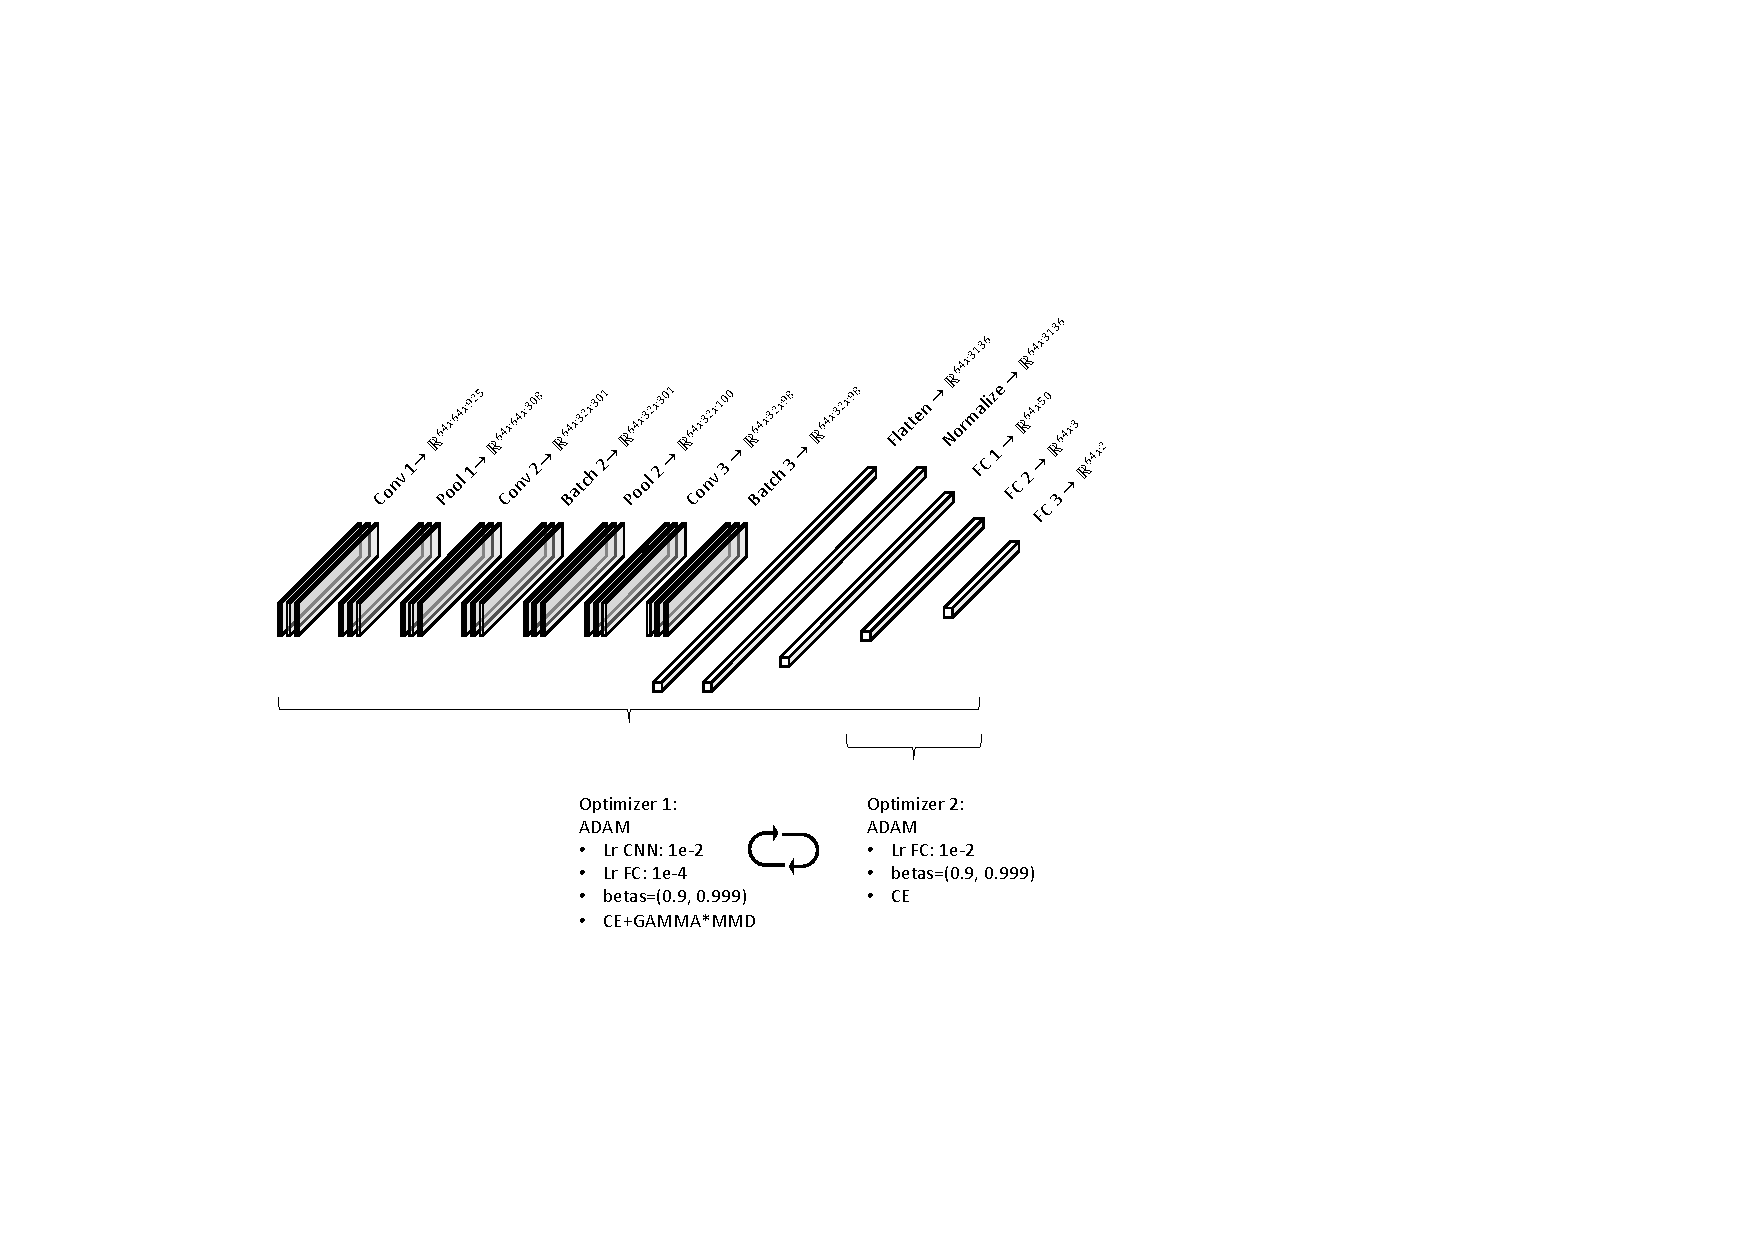
\includegraphics[width=1\textwidth]{proposed_model.pdf}
  \caption {Proposed model} \label{fig:proposed_model}
\end{figure}


\subsection{Proposed Training with MMD- and CE-Loss} \label{sec:Proposed_training}

In a first step, the data used for the training, is pre-processed. In the course of that, the dataloader separates the data in shorter sequences of length 1024. These windows, which can include several of the recorded 49 signals, are fed to the model as single samples. The sequenced signals are cleaned from Nan values and synchronized afterwards. Separate source and target domain dataloader split the corresponding datasets in four different parts: MMD-Training (40\%), CE-Training (20\%), Validation (20\%) and Testing (20\%). Other pre-processing steps, like wavelet transforms, can easily be added to the dataloader. The repetitive training of the model is visualized in fig. \ref{fig:Training_Process_MMD}. The model training is separated in two phases. In a first phase, a weighted average of CE- and MMD-loss is used to optimize the whole network: 
\begin{equation}
    \mbox{Total Loss} = \mbox{Source CE-Loss} + \mbox{GAMMA} \cdot \mbox{MMD-Loss}, 
\end{equation}
where GAMMA is a hyperparameter balancing the influence of the CE- and MMD-loss, which needs to be defined beforehand. Different learning rates in the feature extractor and classifier allow the training intensity to be adjusted separately for the different modules. In this phase an ADAM optimizer is applied with a learning rate of 1e-2 in the layers Conv1 - FC1 and a learning rate of 1e-4 in the layers FC2 - FC3. In a second phase, just the CE-loss is applied to optimize the layers FC2 - FC3. Again an ADAM optimizer with a learning rare of 1e-2 is used. In both optmization steps the beta values are 0.9 and 0.999. Two-thirds of the training data is used in the first and one-third in the second train phase. The application of two different optimizer is visualized in fig. \ref{fig:proposed_model}. The MMD-loss estimates the domain discrepancy in the latent feature maps of the neural network. The MMD-loss facilitates the extraction of domain invariant features. The domain discrepancy is measured as squared distance between the distribution kernel embeddings in the reproducing kernel Hilbert space (RKHS). The kernel choice is of great importance for the performance of the MMD-loss. By combining several RBF kernels with bandwidth parameters 1, 2, 4, 8, 16, the model training profits from their individual strength. The source and target samples are randomly coupled up and processed by the MMD-loss. The classes of these samples are not considered in the MMD-loss. Therefore, the MMD-loss minimizes the domain discrepancy between source and target domain of different and equal classes. The MMD-loss is applied in several layers of the feature extractor and classifier. The source CE-loss optimizes the model to increase the accuracy on the source domain. Fig. \ref{fig:MMD_Loss_and_CE_loss} symbolically shows how the MMD and the source CE-loss is applied in different layers of the model. In general, the training is repeated until the maximum number of epochs is reached. After the training is completed, the model can be used to predict the BSD health condition state of unseen target domain samples. 



\begin{figure}[H]
  \centering
  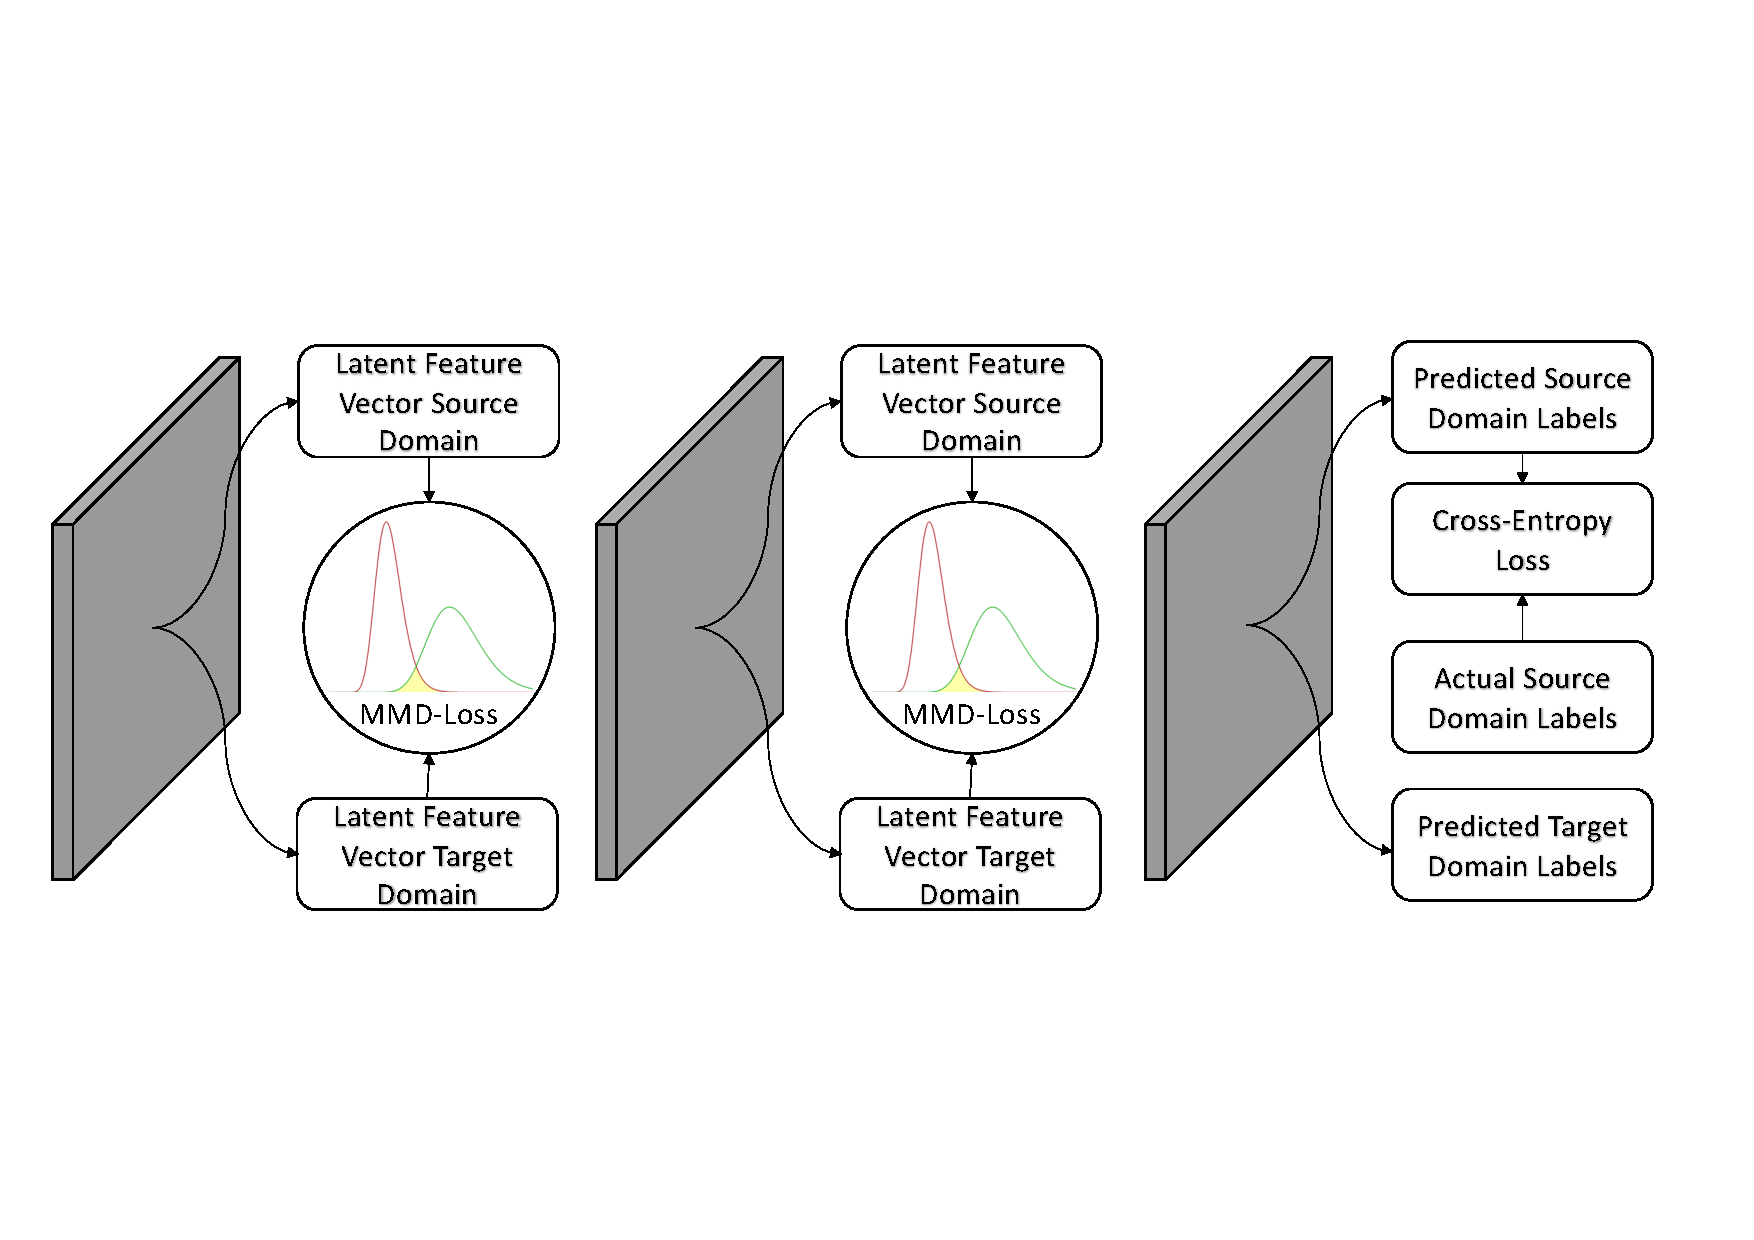
\includegraphics[width=1\textwidth]{MMD_loss_visualization.pdf}
  \caption {CE- and MMD-loss in neural networks} \label{fig:MMD_Loss_and_CE_loss}
\end{figure}

\begin{figure}[H]
  \centering
  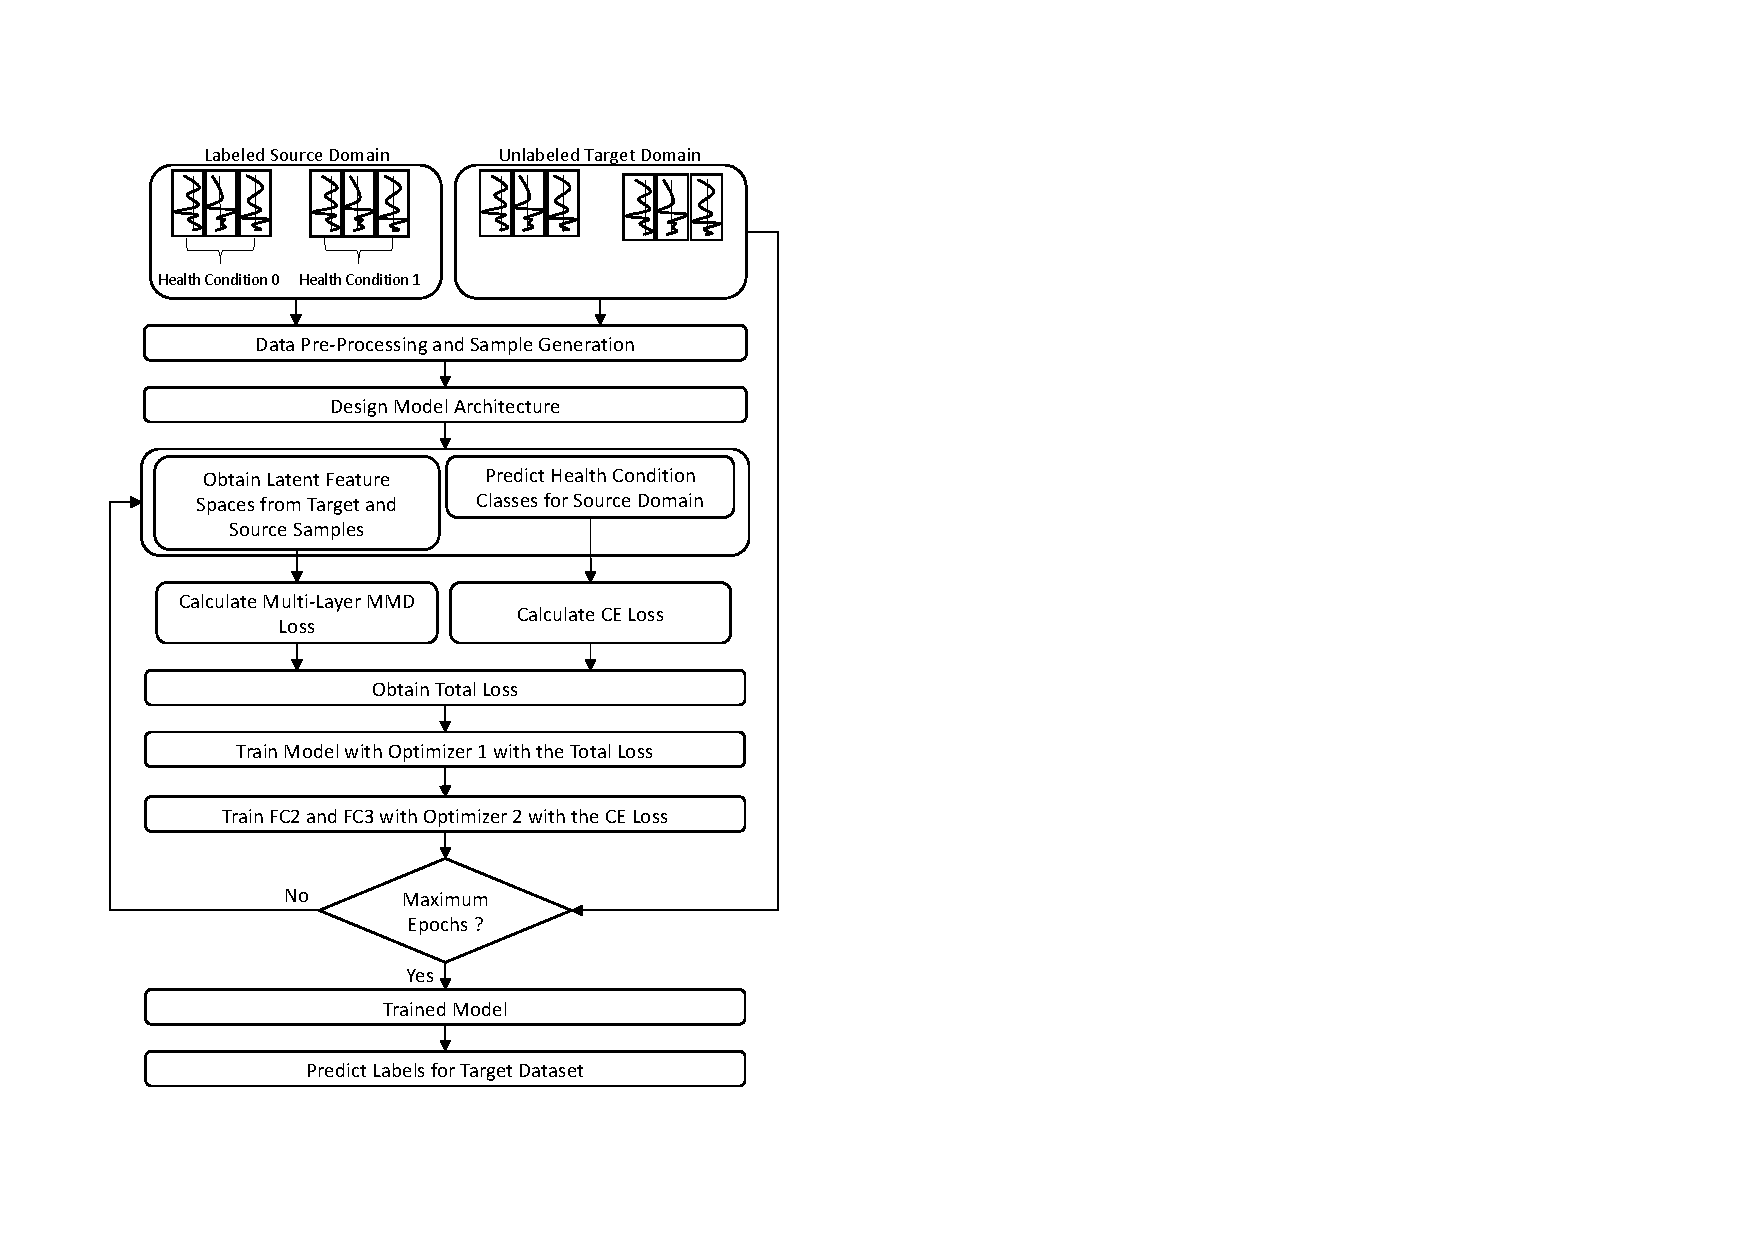
\includegraphics[width=0.8\textwidth]{training_process_mmd.pdf}
  \caption {Model training} \label{fig:Training_Process_MMD}
\end{figure}

